\subsection{Anvendelighet}
\label{chp: anvendelighet}

Generelt kan man definere noe som anvendelig dersom det er funksjonelt, effektivt og tilfredsstillende. Et system er funksjonelt når det anses som nyttig av brukeren, det må dermed svare til de forventningene brukeren har om hva det skal gjøre, og faktisk gjøre det. Effektivitet kan måles som hvor raskt en er i stand til å utføre en oppgave med så lite feil som mulig. Systemets grensesnitt kan eksempelvis variere i kompleksitet ved at oppgaver kan utføres i ett eller flere trinn.  
Det er vanskelig å konkretisere hva som gjør et system tilfredsstillende for en bruker, dette kan være individuelt og er en følelsesmessig respons ved bruk systemet. Ofte vil god design være avgjørende for om en bruker opplever systemet på en god måte, forutsett at det også er funksjonelt og effektivt. Designere av grensesnitt har gjennom årene kommet frem til en rekke reningslinjer for god design av skjermbilder. Disse er ofte blitt kritisert for å være både for spesifikke og ufullstendige \cite{mmi}. Det er derfor avgjørende å utvikle med en forståelse for hva slags informasjon brukeren trenger og hvordan denne skal presenteres \cite{Ebright10}. 

\noindent
\subsubsection{Gestaltprinsippene}
Gestaltprinsippene har sitt navn fra det tyske \emph{gestalten}, som betyr "å forme". Prinsippene blir ofte referert til som lover, og det finnes mange varianter utviklet av forskjellige psykologer, men de har til felles at de forklarer hvordan vi organiserer visuelle intrykk i områder og strukturer. Disse ble i utgangspunktet brukt til å foreslå hvordan statiske visuelle elementer burde presenteres for effektive resultater\cite{Chang02}. Chang, Dooly og Tuovien (2002) identifiserer og presenterer elleve prinsipper med betydelig relevans for design av skermbilder. 

\noindent
Prinsippet om \emph{balanse og symetri}: Visuelle objekter som ikke er balansert vil synes ufullstendig. Når visuell "vekt" er plassert jevnt på hver side av en akse vil vi få en psykologisk følelse av likevekt.

\noindent
Prinsippet om \emph{forlengelse}: Øyet har et instingt til å følge linjer i synsfeltet.

\noindent
Prinsippet om \emph{lukkethet}: Åpne figurer til fremstå som ufullstandige, og vi vil ubevisst prøve å lukke formen for at den skal gi mening.

\noindent
Prinsippet om \emph{figur - bakgrunn}: Vi skiller automatisk mellom forgrunn og bakgrunn. Endringer i forgrunn- og bekgrunnfarge kan føre til at vi ser forskjellige figurer, selv om bildet er det samme. som i figur \ref{forgrunn_bakgrunn}

\begin{figure}
\centering
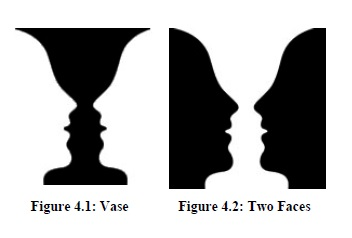
\includegraphics[scale=1]{figure-ground.jpg}
\caption{Her ser vi hvordan vi oppfatter forskjellige figurer når vi bytter forgrunns- og bekgrunnsfarge}
\label{forgrunn_bakgrunn}
\end{figure}

\noindent
Prinippet om \emph{fokuspunkt}: Fokuspunktet er det punktet vi legger merke til først, og dette vil være vårt utgangspunkt for hvordan, og i hvilken rekkefølge vi ser resten av bildet. Som eksempel vil et element som distinkt skiller seg fra resten fange vår oppmerksomhet først.

\noindent
Prinsippet om \emph{isomorft samsvar}: Vi tolker bildet med utgangspunkt i våre erfaringer. Derfor er det ikke gitt at et bilde eller symbol vi gi samme mening for alle.

\noindent
Prisnippet om \emph{god form}: Vi vil gjøre en så god figur ut fra det vi ser som mulig. En god form er et enkelt design eller en symetrisk utforming.

\noindent
Prinsippet om \emph{nærhet}: Vi vil oppfatte objekter som er plassert nær hverandre, adskilt fra andre som en gruppe, og anta at de er relatert til hverandre på noen måte.

\noindent
Prinsippet om \emph{likhet}: Lignende objekter vil ha samme funksjon som objekter plassert nær hverandre, og vi vil se dem som en gruppe, med antagels om realsjon.

\noindent
Prinsippet om \emph{enkelhet}: Underbevisstheten vår prøver å forenkle det vi ser til noe vi kjenner igjen. Kompleks grafikk med mye unødvendige elementer kan føre til at vi trekker utilsiktede konklusjoner.

\noindent
Prinsippet om \emph{harmoni}: Impliserer at det finnes en kongruens mellom elementer i et design. De kan se ut som om de hører sammen som om det er en visuell knytning mellom dem som gjør at de kommer sammen.

\noindent
Forskning viser at andvendelse av disse elleve prinsippene er hensiktsmessig for design av skjermbilder i større eller mindre grad \cite{Chang02}.

\noindent
\subsubsection{Konseptuelle modeller, begrensninger og "affordance"}

\noindent
Hvordan vi forstår hvordan vi skal bruke en gjenstand første gang vi ser den beror på tre dimensjoner: konseptuell modell, begrensniner og "affordance". Ordet "affordance" ble innført av psykologen J. J. Gibson. Det finnes ingen norsk oversettelse, men begrepet refererer til hva slags handling en gjenstand signaliserer når du ser den for første gang.\cite{Norman99}

\noindent
Vi skiller mellom ekte affordance og oppfattet affordance, hvor det først og fremst er oppfattet affordance vi kan kontrollere i skjermdesign. Ekte affordance vil med tanke på datamaskiner være tastatur, skjerm, knapper og musepeker som signaliserer handlinger som berøring, peking, trykking og å se på. Ekte affordance finnes alstå uavhengig av hva som vises på skjermen. Det som vises på skjermen er visuelle tilbakemelinger for å vise oss hva vi kan gjøre, eller oppfattet affordance.\cite{Norman99}

\noindent
Affordance blir ofte forvekslet med begrensninger og konvensjoner, også kallt kulturelle begresninger. Vi kan si å ha tre typer begrensninger: (1) Fysiske begrensninger, som har sammenheng med ekte affordance. et eksempel på dette kan være at det er ikke mulig å flytte musepekeren til utenfor skjermen. (2) Logiske begrensninger er sterkt knyttet til en god konseptuell modell. Det er blandt annet hvordan brukeren vet at den må skrolle for å se resten av siden. (3) Kulturelle begrensninger deles av en gruppe og er tillært, som hva det betyr når markøren skifter form. En konvensjon er en begrensning som forbyr noe og oppfordrer til noe annet. Det er en kulturell begrensning som har utvikle seg over tid. Der affordanve viser til forholdet mellom bruker og objekt, konvensjoner er tilfeldige, kunstige og tillært.\cite{Norman99}

\noindent
Spesielt logiske og kulturelle begrensninger er sterke virkemidler i forbindelse med skjermdesign da designere er mer opptatt av hva brukerene ser som mulig fremfor hva som er sant. Tilbakemeldinger og reaksjoner fra skjermen hjelper oss å forstå hva vi kan og skal gjøre, men er konvensjoner, og ikke affordance.\cite{Norman99}